% \documentclass{article}
\documentclass[11.5pt,a4paper]{article}
\usepackage{graphicx} % Required for inserting images
\usepackage{empheq}

\usepackage{amssymb}

\usepackage{amsmath, bm}


\begin{document}


\section*{\centering \LARGE Beam Behavior with Concentrated Load on Elastic Foundation \vspace{0.5em}}

\section*{\centering \large Linear Theory of Elasticity}

\textbf{The system of field equations:}



Given, $T$ = Piola-Kirchhoff Stress tensor, C = Elasticity tensor, $\epsilon$ = strain, u = displacement, $b_0$ = Body force per unit \textit{mass} (unit volume = density * unit mass), $\nabla_{X}\cdot T$ = Material divergence of Piola-Kirchhoff Stress tensor. The system of field equations for elastic body within the framework of linear theory:

\begin{empheq}[box=\fbox]{align*}
    T &= C[\epsilon]  & \text{(Stress-Strain Law)} \\
    \epsilon &=  \frac{1}{2}(\nabla u + \nabla u^{T}) & \text{(Strain-Displacement relation)} \\ 
    \rho_{0}\frac{\partial^{2} u}{\partial t^2} &=  \nabla_{X} \cdot T + \rho_{0} b_{0} & \text{(Equation of Motion)}
\end{empheq}

\begin{itemize}
    \item The strain-displacement relation, derived from \textit{Kinematics}, represents the linear function of displacement used as the strain measure.
    \item The stress measure is obtained under the assumption that the displacement gradient is small. Therefore, stress measures such as Cauchy's stress $\tau$ and Piola-Kirchhoff stress $T$ are approximately equal i.e $\tau \approx T$.
    \item The governing equation for linear elasticity is the Cauchy's equation of motion with the stress tensor represented by the Piola-Kirchhoff stress.
\end{itemize}

Given ${C , \rho_0, b_0}$, the field equation represents a linear system of partial differential equations for the fields ${u, \epsilon, T}$. When the body is isotropic, i.e., materials exhibit the same mechanical response to forces or deformations regardless of the direction in which those forces or deformations are applied. The constitutive relation is given by:
\hspace{-0.5em}
\begin{align*}
     T  &= \lambda(tr \epsilon)I + 2\mu \epsilon  & \text{($\lambda$ and $\mu$ are Lame Constant)}
\end{align*}


\textbf{Homogeneous and Isotropic Body:}

Assume that body is homogeneous and isotropic, ${\rho_0, \mu,\lambda}$ are constants,


\begin{empheq}[box=\fbox]{align*}
    \mu &  & \text{(Shear Modulus)} \\
    \kappa &= \lambda + \frac{2}{3}\mu   & \text{(Bulk Modulus)} \\ 
    E &= \frac{\mu(2\mu + 3\lambda)}{(\mu + \lambda)}   & \text{(Young's Modulus)} \\ 
    \nu &= \frac{\lambda}{2(\mu + \lambda)}   & \text{(Poisson's Ratio)} 
\end{empheq}

\textbf{Relation between $E$ and $\nu$:}
\begin{align*}
    \epsilon &= \frac{1}{E}[(1+ \nu)T - \nu(tr T)I]
\end{align*}



\section*{\centering \large Differential Equation of the Deflection Curve}

\textbf{Deflection Curve Differential Relations:}

\begin{figure}[h]
        \centering 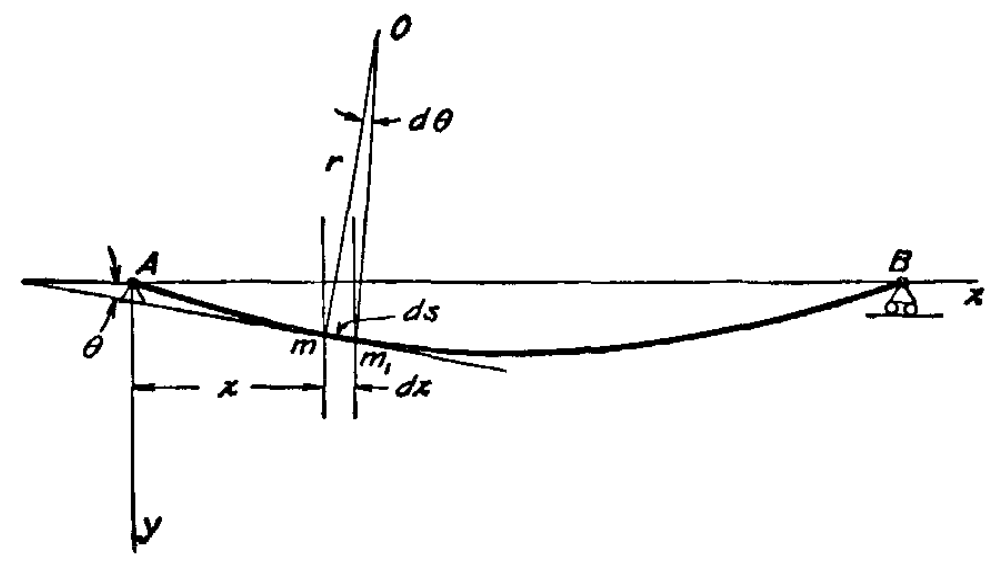
\includegraphics[width=0.9\textwidth]{defl.png}
\end{figure}



Given, r = Radius of Curvature, $I_{z}$ = Moment of Inertia, E$I_{z}$ = Flexural Rigidity, $\partial s$, $\partial \theta$  = distance and Angle between m and m1.
\begin{align*} 
    \frac{1}{r} &= \frac{M}{EI_{z}}  & \text{(Radius of Curvature relation)}
\end{align*}

\textbf{\textit{To a positive increment $\partial s$ corresponds a negative $\partial \theta$}}.

\begin{align*} 
    {\partial s} &= - r {\partial \theta} & 
    \frac{1}{r} &= - \frac{\partial \theta}{\partial s}\\
    {\partial s} &\approx \partial x  & &
    \theta = \frac{\partial y}{\partial x}
\end{align*}

Substituting the above relations to the Radius of curvature equation, 
\begin{align*} 
    \frac{1}{r} &=  \frac{\partial}{\partial x}(\frac{\partial y}{\partial x}) = - \frac{\partial^{2} y}{\partial x^2} = \frac{M}{EI_{z}} \\
    M &= - EI_{z}\frac{\partial^{2} y}{\partial y^2}
\end{align*}

% Strain relations from Hooke's Law we can,
% \begin{align*} 
%     \epsilon_{x} &= \frac{y}{r} & \text{(strain)}\\
%     \sigma_{x} &= \frac{Ey}{r} & \text{(Stress)}\\
%     \sigma_{x} &= \frac{My}{I_{z}} & \text{(Equation for Stress)} 
% \end{align*}

Hence, by comparing the relations the following differential equations are employed:


\begin{empheq}[box=\fbox]{align*}
    M &= - EI_{z}\frac{\partial^{2} y}{\partial x^{2}} & \text{(Bending Moment)} \\
    V &= - EI_{z}\frac{\partial^{3} y}{\partial x^{3}} & \text{(Shearing Force)} \\
    q &= EI_{z}\frac{\partial^{4} y}{\partial x^{4}} & \text{(Load Intensity)}
\end{empheq}

\newpage

\section*{\centering \large The General Solution: Infinite Beam on an Elastic Foundation (Unloaded)}

\textbf{Assumption:} The reaction forces of the elastic foundation vary proportionally with the deflection of the beam at each point. (E.Winkler) 
\vspace{1em}

\raggedright\textbf{Differential Equation of Elastic foundation:} 

\begin{itemize}
     \item Consider a straight beam supported by an elastic medium, which is subjected to vertical load P (transverse load). This load causes the beam to deflect, resulting in continuously distributed reaction force between beam and the elastic foundation. 
     \item The reaction per unit length on beam, due to the stiffness of the elastic foundation, is proportional to the deflection of the beam $y$ and the constant $k$, known as the \textit{modulus of the foundation} ($k$ includes the effect of width of the beam). The intensity $q$ of the reaction forces on beam is given as: $q = ky$.
     
     \item We assume $q$ is positive when the foundation pushes the beam upward. Consequently, when the deflection $y$ is $positive$ (directed downwards), $q$ is taken as $positive$ (foundation is compressed and pushes up the beam). Conversely, when the deflection $y$ is $negative$ (directed upwards), $q$ is taken as $negative$ (tension produced in the foundation and pulls down the beam).
\end{itemize}

\raggedright\textbf{General Solution:} 

In the case where a beam rests on an elastic foundation without being subjected to any external loads, the only force acting on the beam is the continuously distributed reaction from the elastic foundation. Considering the sign conventions, the intensity on the beam can be expressed as:

\begin{align*} 
q &= -ky & EI_z \frac{d^{4}y}{dx^{4}} &= -ky
\end{align*}

By introducing the notation

\begin{align*} 
\beta &= \sqrt[4]{\frac{k}{4EI_{z}}}
\end{align*}

The general solution for a beam on an elastic foundation (Unloaded) is given by:
\begin{empheq}[box=\fbox]{align*}
\bm{y =  e^{\beta x}(A cos \beta x + B sin \beta x) + e^{-\beta x}(C cos \beta x + D sin \beta x)}
\end{empheq}

Where: \(y\) represents the deflection of the beam, \(A\), \(B\), \(C\), and \(D\) are constants determined by the boundary conditions of the specific problem, and \(\beta\) is the foundation constant or the \textit{characteristic} of the system, it includes the flexural rigidity. \(\beta\) depends on the elastic properties of the foundation and the beam.


\section*{\centering \large Case Study: Single Concentrated Load at origin on Infinitely Long Beam with Elastic Foundation.}

 The solutions for the response of a beam supported by an elastic foundation and loaded by a concentrated load can be obtained using the \textit{Method of Superposition}.
\begin{figure}[h]
        \centering 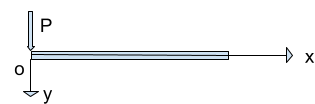
\includegraphics[width=0.5\textwidth]{conc.png}
\end{figure}

Consider a semi-infinite beam resting on an elastic foundation with a concentrated load P at the origin. As x approaches a large positive value, the deflection y tends to zero, causing the curvature to vanish. Consequently, the constants A and B in the general solution will be \textit{zero}. Therefore, the general solution for the deflection curve for right part ($x>0$) can be expressed as:
\begin{empheq}[box=\fbox]{align*}
    \bm{y =  e^{-\beta x}(C cos \beta x + D sin \beta x),} & \quad \bm{x \ge 0}
\end{empheq}

\raggedright\textbf{Boundary Conditions: Determination of C and D} 

\textbf{Assumptions:}
\begin{itemize}

     \item The slope of the beam remains zero under the load due to symmetry.
     \item Half of the load P is supported by the elastic foundation under the half of the beam specified by positive values of $x$.
     \item The other half of the load P is supported by the elastic foundation where $x < 0$. 
\end{itemize} 


Therefore, from the conditions of symmetry,
\begin{align*}
    & \left(\frac{dy}{dx}\right)_{x=0} = 0 \quad :=  \quad -(C-D) = 0 \quad := \bm{[C = D]}
\end{align*}

Rearranging the equation for deflection curve for $x \ge 0$,
\begin{align*}
    \bm{y =  Ce^{-\beta x}(cos \beta x + sin \beta x)}
\end{align*}


The constant \textbf{C} in the equation can be determined by ensuring that the sum of the reaction forces maintains equilibrium with the load \textbf{P}.

\begin{align*}
    P &= 2 \int_{0}^{\inf} ky \, dx\\
    &= 2kC \int_{0}^{\inf} e^{-\beta x}(cos \beta x + sin \beta x) \, dx \\
    &= 2kC (\frac{1}{\beta})
\end{align*} 

Therefore, we can express \textbf{C} as:
\begin{empheq}[box=\fbox]{align*}
    \bm{C = \frac{P\beta}{2k}}
\end{empheq} 

Substituting the boundary condition (\textbf{C}) into the \textbf{solution for the deflection curve for the right part ($\bm{x\ge0}$)}, we have:

\begin{empheq}[box=\fbox]{align*}
    \bm{y =  \frac{P\beta}{2k}e^{-\beta x}(cos \beta x + sin \beta x)}
\end{empheq}

Notations:
\begin{align*}
    \varphi &= e^{-\beta x}(cos \beta x + sin \beta x) & \alpha &= e^{-\beta x}(cos \beta x) \\
    \psi &= -e^{-\beta x}(sin \beta x - cos \beta x) & \zeta &= e^{-\beta x}(sin \beta x)
\end{align*}

Using the notations, we can express the deflection, slope, bending moment, and shear as:
\begin{empheq}[box=\fbox]{align*}
    y &= \frac{P\beta}{2k}\varphi(\beta x)  & \text{(Deflection)} \\ 
    \theta &=  -\frac{P\beta^{2}}{k}\zeta(\beta x) & \text{(Slope)} \\ 
    M &=  \frac{P}{4\beta}\psi(\beta x) & \text{(Bending Moment)} \\
    V &= -\frac{P}{2}\alpha(\beta x) & \text{(Shear)} 
\end{empheq}

The maximum deflection and maximum bending moment occur at the origin ($x=0$), given by:
\begin{empheq}[box=\fbox]{align*} 
    y_{max} &= \frac{P\beta}{2k}  & \text{(Max. Deflection)} \\ 
    M_{max} &=  \frac{P}{4\beta} & \text{(Max. Bending Moment)} 
\end{empheq}

\textbf{Note:} The solution for the deflection curve for the left part ($x<0$) can be obtained by  $\bm{[y(-x)=y(x)]}$ (due to symmetry).

\end{document}
